\section{Experiments}
In this section, we validate the proposed solution by training vision transformers with additional \texttt{[reg]} register tokens.
We evaluate the effectiveness of our approach by a quantitative and qualitative analysis.\old{ of the artefacts in feature maps after training.}
We then ablate the number of registers used for training, to check that they \new{do not} cause a performance regression, evaluate an unsupervised object discovery method atop our features and finally provide a qualitative analysis of the patterns learnt by the registers.


\subsection{Training algorithms and data}
\label{sec:algos}
As the proposed solution is a simple architectural change, we can easily apply it to any training procedure. 
We try it on three different state-of-the-art training methods for supervised, text-supervised, and unsupervised learning, shortly described below.

\textbf{DEIT-III}~\citep{touvron2022deit} is a simple and robust supervised training recipe for classification with ViTs on ImageNet-1k and ImageNet-22k.
We choose this method as an example of label-supervised training as it is simple, uses the base ViT architecture, achieves strong classification results, and is easy to reproduce and modify with our improvements. 
We run this method on the ImageNet-22k dataset, using the ViT-B settings, as provided in the official repository~\footnote{\url{https://github.com/facebookresearch/deit}}.

\textbf{OpenCLIP}~\citep{ilharco_gabriel_2021_5143773} is a strong training method for producing text-image aligned models, following the original CLIP work. 
We chose this method as an example of text-supervised training because it is open-source, uses the base ViT architecture, and is easy to reproduce and modify with our improvements. 
We run the OpenCLIP method on a text-image-aligned corpus based on Shutterstock that includes only licensed image and text data. 
We use a ViT-B/16 image encoder, as proposed in the official repository~\footnote{\url{https://github.com/mlfoundations/open_clip}}.

\textbf{DINOv2}~\citep{oquab2023dinov2} is a self-supervised method for learning visual features, following the DINO work.
We apply our changes to this method as it is the main focus of our study. 
We run this method on ImageNet-22k with the ViT-L configuration.
We use the official repository~\footnote{\url{https://github.com/facebookresearch/dinov2}}.



\subsection{Evaluation of the proposed solution}
As shown in Fig.~\ref{fig:pullfig_beforeafter}, we get rid of the artifacts by training models with additional register tokens.
In the appendix, we provide additional qualitative results for more images in Fig.~\ref{fig:supmat_pagefig_attmaps_beforeafter}.
In order to quantitatively measure this effect, for each model, we probe the norm of features at the output of the model. 
We report these norms for all three algorithms with and without registers in Fig.~\ref{fig:norm_distrib_before_after}.
We see that when training with registers, models do not exhibit large-norm tokens at the output, which confirms the initial qualitative assessment.

\begin{figure}[t]
  \centering
  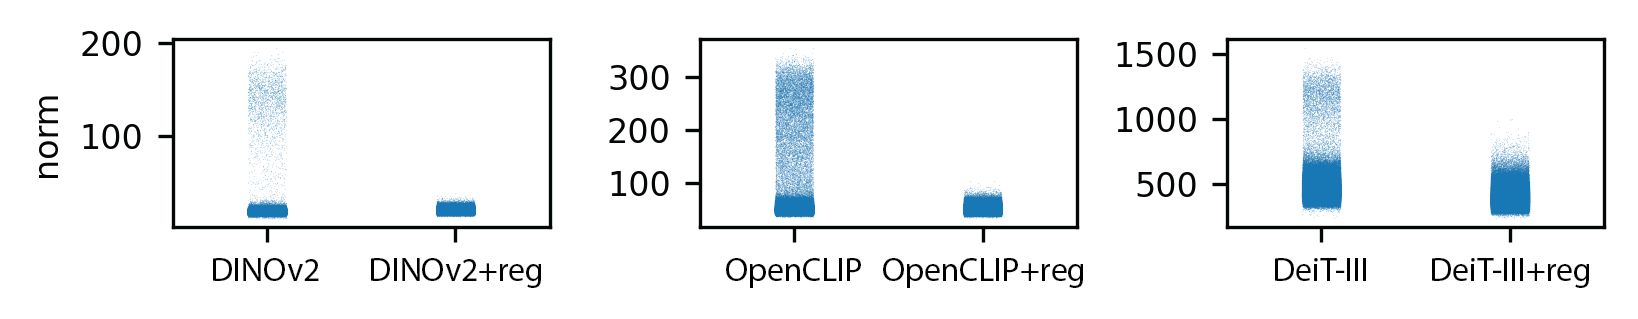
\includegraphics[width=\textwidth]{resources/fig_norm_distrib_before_after_stripplot-2.png}
  \caption{
    Effect of register tokens on the distribution of output norms on DINOv2, OpenCLIP and DeiT-III.
    Using register tokens effectively removes the norm outliers that were present previously.
  }
  \label{fig:norm_distrib_before_after}
\end{figure}


\textbf{Performance regression.}
In the previous section, we \new{have shown} that the proposed approach removes artifacts from local feature maps.
In this experiment, we want to check that the use of register tokens does not affect the representation quality of those features.
We run linear probing on ImageNet classification, ADE20k Segmentation, and NYUd monocular depth estimation.
We follow the experimental protocol outlined in~\cite{oquab2023dinov2}.
We summarize the performance of the models described in Sec.~\ref{sec:algos} with and without register tokens in Table~\ref{tab:linear}.
We see that when using registers, models do not lose performance and sometimes even work better.
For completeness, we also provided the zero-shot classification performance on ImageNet for OpenCLIP (Table~\ref{tab:zero-shot}), which remains unchanged.
Please note that the absolute performance of our OpenCLIP reproduction is lower due to the data source we used.

\begin{table}[t]
  \centering
  \subcaptionbox{Linear evaluation with frozen features.\label{tab:linear}}{
    \centering
    \begin{tabular}{@{}l c ccc@{}}
    	\toprule
    	            && ImageNet & ADE20k  & NYUd \\
                  && Top-1  & mIoU    & rmse $\downarrow$ \\
    	\midrule
      DeiT-III      && 84.7   & 38.9   & 0.511    \\
      DeiT-III+reg  && 84.7   & 39.1   & 0.512    \\
      \midrule
      OpenCLIP      && \internaldeadlinemodif{78.2}   & \internaldeadlinemodif{26.6}   & \internaldeadlinemodif{0.702}    \\
      OpenCLIP+reg  && \internaldeadlinemodif{78.1}   & \internaldeadlinemodif{26.7}   & \internaldeadlinemodif{0.661}    \\
      \midrule
      DINOv2        && 84.3 & 46.6 & 0.378 \\
      DINOv2+reg    && 84.8 & 47.9 & 0.366 \\
    	\bottomrule
    \end{tabular}
  }
  \hspace{3em}
  \subcaptionbox{Zero-shot classification.\label{tab:zero-shot}}{
    \begin{tabular}{@{}l c c@{}}
    	\toprule
    	            && ImageNet \\
                  && Top-1  \\
    	\midrule
      OpenCLIP      && \internaldeadlinemodif{59.9}    \\
      OpenCLIP+reg  && \internaldeadlinemodif{60.1}    \\
    	\bottomrule
    \end{tabular}
  }
  \caption{
    Evaluation of downstream performance of the models that we trained, with and without registers.
    We consider linear probing of frozen features for all three models, and zero-shot evaluation for the OpenCLIP model.
    We see that using register not only does not degrade performance, but even improves it by a slight margin in some cases.
  }  
  \label{tab:downstream}
\end{table}




\textbf{Number of register tokens.}
As described in Sec.~\ref{sec:hypothesis}, we propose alleviating the feature maps' artifacts by adding register tokens. 
In this experiment, we study the influence of the number of such tokens on local features and downstream performance.
We train DINOv2 ViT-L/14 models with 0, 1, 2, 4, 8 or 16 registers.
In Fig.~\ref{fig:scores_n_reg}, we report the results of this analysis.
In Fig.~\ref{fig:scores_n_reg}\textbf{(top)}, we qualitatively study the attention maps and observe that the visible artifacts disappear when adding at least one register.
We then examine in Fig.~\ref{fig:scores_n_reg}\textbf{(bottom)} performance on downstream evaluation benchmarks, following the protocol from~\cite{oquab2023dinov2}.
There seems to be an optimal number of registers for dense tasks, and adding one brings most of the benefit.
This optimum is likely explained by the disappearance of artifacts, leading to better local features.
On ImageNet, however, performance improves when using more registers.
In all our experiments, we kept $4$ register tokens.

\begin{figure}[t]
  \centering
  \begin{tabular}{*{7}{>{\centering\arraybackslash}m{0.135\textwidth}@{}}}
    Input & 0 \texttt{[reg]} & 1 \texttt{[reg]} & 2 \texttt{[reg]} & 4 \texttt{[reg]} & 8 \texttt{[reg]} & 16 \texttt{[reg]} \\
    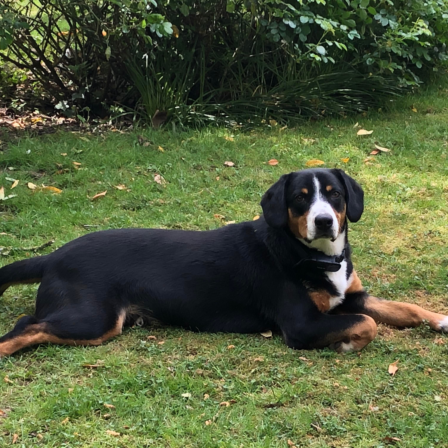
\includegraphics[width=0.13\textwidth]{resources/230916_attmap_vs_n_reg/pyrrhus_orig.png} &
    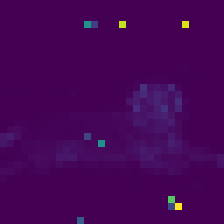
\includegraphics[width=0.13\textwidth]{resources/230916_attmap_vs_n_reg/100cc_pyrrhus_0reg.png} &
    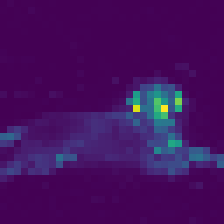
\includegraphics[width=0.13\textwidth]{resources/230916_attmap_vs_n_reg/100cc_pyrrhus_1reg.png} &
    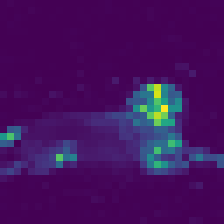
\includegraphics[width=0.13\textwidth]{resources/230916_attmap_vs_n_reg/100cc_pyrrhus_2reg.png} &
    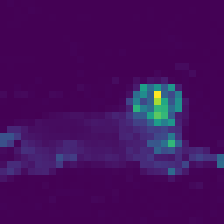
\includegraphics[width=0.13\textwidth]{resources/230916_attmap_vs_n_reg/100cc_pyrrhus_4reg.png} &
    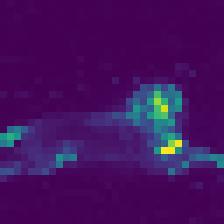
\includegraphics[width=0.13\textwidth]{resources/230916_attmap_vs_n_reg/100cc_pyrrhus_8reg.png} &
    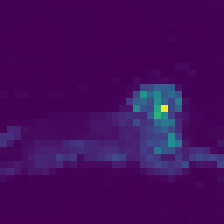
\includegraphics[width=0.13\textwidth]{resources/230916_attmap_vs_n_reg/100cc_pyrrhus_16reg.png}
  \end{tabular} \\
  \vspace{0.3em}
  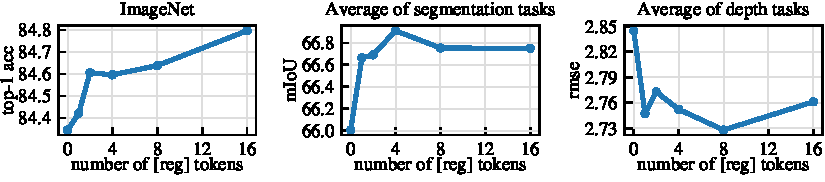
\includegraphics{resources/ablation_n_reg.pdf}
  \caption{
    Ablation of the the number of register tokens used with a DINOv2 model.
    \textbf{(top)}: qualitative visualization of artifacts appearing as a function of number of registers. 
    \textbf{(bottom)}: performance on three tasks (ImageNet, ADE-20k and NYUd) as a function of number of registers used.
    While one register is sufficient to remove artefacts, using more leads to improved downstream performance.
  }
  \label{fig:scores_n_reg}
\end{figure}




\subsection{Object discovery}\label{sec:obj_discovery}
Recent unsupervised object discovery methods rely on the quality and smoothness of local feature maps~\citep{simeoni2021localizing,wang2023cut}.
By leveraging DINO~\cite{caron2021emerging}, these methods \new{have significantly} surpassed the previous state of the art\old{ significantly}. 
However, the algorithm leads to poor performance when applied to modern backbones such as DINOv2~\cite{oquab2023dinov2} or supervised ones~\cite{touvron2022deit}.
We posit that this can be alleviated by the method proposed in this work.
We run LOST~\citep{simeoni2021localizing} on features extracted from backbones trained using the algorithms described in Sec.\ref{sec:algos} with and without registers. 
We run object discovery on PASCAL VOC 2007 and 2012 and COCO 20k.
We use values for DeiT and OpenCLIP, and for DINOv2, we use keys.
Because the output features may have different conditioning, we manually add a bias to the gram matrix of features.
The results of this experiment are presented in Table~\ref{tab:lost}.
For DINOv2 and DeiT-III, adding registers significantly improves the discovery performance. 
For OpenCLIP, the performance is slighty worse with registers (see Sec.~\ref{sec:appendix-lost} for analysis).
The performance of DINOv2 on VOC2007 still does not match that of DINO as reported by~\citet{simeoni2021localizing} ($61.9$ corloc).
However, the model with registers gets an improvement of $20.1$ corloc ($55.4$ versus $35.3$).

\begin{table}[t]
  \centering
  \begin{tabular}{@{}l c ccc@{}}
  	\toprule
  	            && VOC 2007 & VOC 2012  & COCO 20k \\
  	\midrule
    DeiT-III      && 11.7 & 13.1 & 10.7 \\
    DeiT-III+reg  && 27.1 & 32.7 & 25.1 \\
    \midrule
    OpenCLIP      && \new{38.8} & \new{44.3} & \new{31.0} \\
    OpenCLIP+reg  && \new{37.1} & \new{42.0} & \new{27.9} \\
    \midrule
    DINOv2        && 35.3 & 40.2 & 26.9 \\
    DINOv2+reg    && 55.4 & 60.0 & 42.0 \\
  	\bottomrule
  \end{tabular}
  \caption{
    Unsupervised Object Discovery using LOST~\citep{simeoni2021localizing} on models with and without registers.
    We evaluated three types of models trained with various amounts of supervision on VOC 2007, 2012 and COCO.
    We measure performance using corloc.
    We observe that adding register tokens makes all models significantly more viable for usage in object discovery.
  }  
  \label{tab:lost}
\end{table}



\subsection{Qualitative evaluation of registers}
In this final experiment, we qualitatively probe for the behavior of register tokens. 
We want to verify if they all exhibit similar attention patterns or whether a differentiation automatically emerges.
To this end, we plot the attention maps of the class and register tokens to patch tokens.
The result of this visualization is shown in Fig.~\ref{fig:slot_attn}.
We see that registers do not have a completely aligned behavior.
Some selected registers exhibit interesting attention patterns, attending to the different objects in the scene.
While nothing enforced this behavior, their activations had some natural diversity.
We leave the study of the regularization of registers for future work.

\begin{figure}[t]
  \begin{tabular}{cccccc}
    Input & \texttt{[CLS]} & \texttt{[reg$_0$]} & \texttt{[reg$_6$]} & \texttt{[reg$_8$]} & \texttt{[reg$_{12}$]} \\
    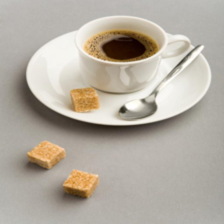
\includegraphics[width=0.13\textwidth]{resources/230913_fig_slot_attn/mug.png} &
    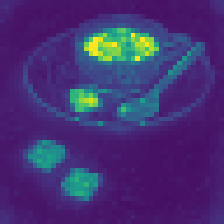
\includegraphics[width=0.13\textwidth]{resources/230913_fig_slot_attn/mug_attn_cls.png} &
    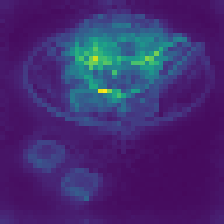
\includegraphics[width=0.13\textwidth]{resources/230913_fig_slot_attn/mug_attn_reg_0.png} &
    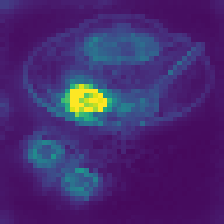
\includegraphics[width=0.13\textwidth]{resources/230913_fig_slot_attn/mug_attn_reg_6.png} &
    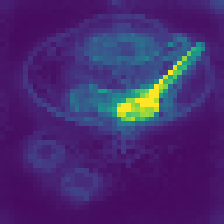
\includegraphics[width=0.13\textwidth]{resources/230913_fig_slot_attn/mug_attn_reg_8.png} &
    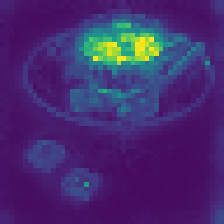
\includegraphics[width=0.13\textwidth]{resources/230913_fig_slot_attn/mug_attn_reg_12.png}
    \\
  \end{tabular}
  \caption{
    Comparison of the attention maps of the \texttt{[CLS]} and register tokens.
    Register tokens sometimes attend to different parts of the feature map, similarly to slot attention \citep{locatello2020object}.
    This behaviour was never required from the model, and emerged naturally from training.
  }
  \label{fig:slot_attn}
\end{figure}



